\documentclass[aspectratio=169,11pt]{beamer}

\usetheme{Madrid}
\usecolortheme{default}
\setbeamertemplate{navigation symbols}{}
\setbeamertemplate{footline}[frame number]
\definecolor{holmblue}{RGB}{0,86,125}
\definecolor{holmgreen}{RGB}{44,125,94}
\definecolor{lightblue}{RGB}{232,243,248}
\setbeamercolor{structure}{fg=holmblue}
\setbeamercolor{frametitle}{fg=holmblue}
\setbeamercolor{block title}{bg=holmblue,fg=white}
\setbeamercolor{block body}{bg=lightblue,fg=black}

\usepackage[T1]{fontenc}
\usepackage[utf8]{inputenc}
\usepackage[english]{babel}
\usepackage{booktabs}
\usepackage{tabularx}
\usepackage{tikz}
\usetikzlibrary{arrows.meta,positioning,fit,shapes.geometric}
\usepackage{hyperref}
\hypersetup{colorlinks=true,urlcolor=holmblue,linkcolor=holmblue}

\title{Urban Freight Microdepots}
\subtitle{State of research, the EU Horizon project NEXTLOGIC,\\
and HOLM's role in Frankfurt}
\author{Research overview based on the provided sources}
\institute{House of Logistics and Mobility (HOLM) context}
\date{November 2026}

\newcommand{\source}[1]{\par\vspace{2pt}{\tiny\textcolor{gray}{Source: #1}}}

\begin{document}

\begin{frame}
  \titlepage
\end{frame}

\begin{frame}{Guiding question and structure}
\begin{block}{Guiding question}
How can urban microdepots support a more efficient, low-emission last mile---and what does NEXTLOGIC add to the evidence base?
\end{block}
\begin{enumerate}
  \item Concept, typologies and expected effects
  \item What the literature and practice show so far
  \item Location planning and data requirements
  \item NEXTLOGIC and the Frankfurt demonstrator
  \item HOLM's role and open research needs
\end{enumerate}
\end{frame}

\begin{frame}{Why microdepots? The urban last-mile problem}
\begin{columns}[T]
\column{0.48\textwidth}
\begin{itemize}
  \item Growing parcel volumes and high delivery density
  \item Congestion, curb-space competition and repeated stop-and-go traffic
  \item Accessibility constraints in historic centres and pedestrian areas
  \item Pressure to reduce emissions, noise and road-safety risks
\end{itemize}
\column{0.48\textwidth}
\begin{block}{Core intervention}
Move the final transshipment point closer to receivers and shift the last leg from vans to cargo bikes or other zero-emission modes.
\end{block}
\begin{block}{Important qualification}
Benefits depend on consolidation, suitable locations, viable operations and stakeholder cooperation; a depot is not an impact guarantee by itself.
\end{block}
\end{columns}
\source{Katsela et al. (2022); Mauch et al., \emph{logSPAZE}; EU Urban Mobility Observatory, “Microhubs as the future of last-mile logistics”.}
\end{frame}

\begin{frame}{A working definition}
\begin{block}{Urban freight microhub}
“A logistics facility where commercial transport providers consolidate goods near the final delivery point and serve a limited spatial delivery area in a dense urban setting.”
\end{block}
\begin{itemize}
  \item It is closer to final customers and smaller in spatial catchment than a conventional urban consolidation centre.
  \item It can enable a mode shift to electric and non-motorised vehicles.
  \item The last mile starts at the microhub; the carrier completes delivery to the receiver.
  \item The term is used alongside \emph{micro-depot}, \emph{micro-consolidation centre} and \emph{city hub}; terminology remains heterogeneous.
\end{itemize}
\source{Katsela, Kourounioti, Thoen, Winkenbach \& de Koster (2022), \emph{Sustainability} 14, 532.}
\end{frame}

\begin{frame}{Typologies: one concept, several operating models}
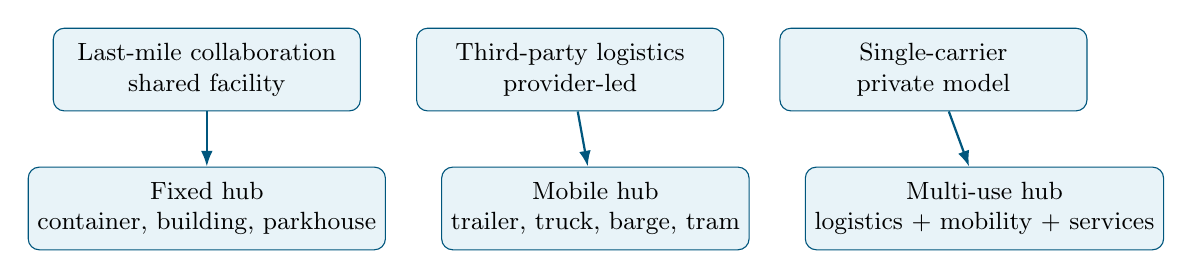
\begin{tikzpicture}[
  node distance=7mm and 7mm,
  box/.style={rounded corners, draw=holmblue, fill=lightblue, align=center,
              minimum width=3.9cm, minimum height=1.05cm, font=\small},
  arrow/.style={-{Latex[length=2mm]}, thick, draw=holmblue}
]
\node[box] (collab) {Last-mile collaboration\\shared facility};
\node[box, right=of collab] (third) {Third-party logistics\\provider-led};
\node[box, right=of third] (private) {Single-carrier\\private model};
\node[box, below=of collab] (fixed) {Fixed hub\\container, building, parkhouse};
\node[box, right=of fixed] (mobile) {Mobile hub\\trailer, truck, barge, tram};
\node[box, right=of mobile] (mixed) {Multi-use hub\\logistics + mobility + services};
\draw[arrow] (collab) -- (fixed);
\draw[arrow] (third) -- (mobile);
\draw[arrow] (private) -- (mixed);
\end{tikzpicture}
\vspace{4mm}
\begin{itemize}
  \item Typology is multidimensional: ownership, partnerships, infrastructure, location, scale and fleet.
  \item Public support and local objectives shape the feasible model.
\end{itemize}
\source{Katsela et al. (2022); HOLM campaign documentation (2021).}
\end{frame}

\begin{frame}{What practice has demonstrated}
\begin{columns}[T]
\column{0.52\textwidth}
\begin{itemize}
  \item German cases cover public parking spaces, parkhouses, former vacant buildings, company sites, containers and mobile solutions.
  \item Examples combine parcel transshipment with charging, workshops, parcel shops, collection points or other urban services.
  \item Shared use can avoid multiple carriers entering the same central area.
  \item The HOLM campaign documented 14 German microdepots as a practice overview, not as a statistically complete sample.
\end{itemize}
\column{0.44\textwidth}
\begin{block}{Observed design principle}
The best-performing concept is context-dependent: a temporary curbside hub, a building-based hub and a mobile hub solve different space and access problems.
\end{block}
\end{columns}
\source{HOLM, \emph{Deutschland sucht das Super-Mikrodepot} (2021); Mauch et al., \emph{logSPAZE}.}
\end{frame}

\begin{frame}{Research evidence: promising, but conditional}
\begin{table}
\small
\begin{tabularx}{\textwidth}{@{}lX@{}}
\toprule
\textbf{Dimension} & \textbf{State of knowledge} \\
\midrule
Environmental & Potential for fewer vehicle kilometres, lower local emissions and quieter deliveries when the last mile shifts to cargo bikes or other clean modes. \\
Operational & Consolidation and shorter tours can improve efficiency, but handling, staffing, charging and time windows create additional costs. \\
Urban & Hubs can improve access to dense areas, yet compete for scarce curb, parking and public-space capacity. \\
Governance & Success depends on carriers, city authorities, property owners, residents and data partners sharing responsibilities. \\
Evidence gap & Many studies are case-based or model-based; long-term, comparable before/after evidence remains limited. \\
\bottomrule
\end{tabularx}
\end{table}
\source{Katsela et al. (2022); Mauch et al., \emph{logSPAZE}; EU Urban Mobility Observatory.}
\end{frame}

\begin{frame}{Location planning: from intuition to multi-criteria models}
\begin{columns}[T]
\column{0.48\textwidth}
\begin{block}{Typical decision variables}
\begin{itemize}
  \item Number, location and capacity of hubs
  \item Assignment of demand zones
  \item Fleet and staff allocation
  \item Access, transfer and routing policy
\end{itemize}
\end{block}
\column{0.48\textwidth}
\begin{block}{Typical objectives}
\begin{itemize}
  \item Cost and service quality
  \item Emissions and vehicle kilometres
  \item Coverage and delivery distance
  \item Robustness under demand and access constraints
\end{itemize}
\end{block}
\end{columns}
\vspace{3mm}
\begin{alertblock}{Recent modelling direction}
\footnotesize Stokkink et al. formulate a mixed-integer model combining truck, metro and micromobility, including hub location, capacity and fleet assignment. Their Madrid case illustrates that multimodal design can outperform a traditional last-mile benchmark, but the optimum depends on demand, hub costs and network access.
\end{alertblock}
\source{Stokkink \& Geroliminis (2025), “On the optimal micro-hub locations in a multi-modal last-mile delivery system”.}
\end{frame}

\begin{frame}{Frankfurt: the data foundation for a location model}
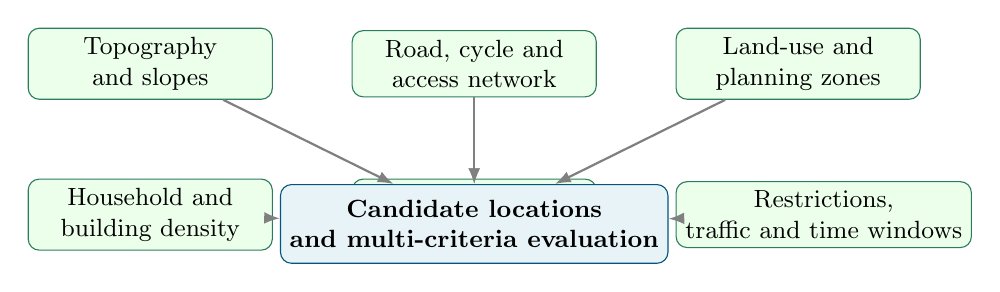
\begin{tikzpicture}[
  every node/.style={font=\small},
  src/.style={rounded corners, draw=holmgreen, fill=green!8, align=center,
              minimum width=3.1cm, minimum height=0.8cm},
  core/.style={rounded corners, draw=holmblue, fill=lightblue, align=center,
               minimum width=4.0cm, minimum height=1.0cm, font=\bfseries\small},
  arr/.style={-{Latex[length=2mm]}, thick, draw=gray}
]
\node[src] (terrain) {Topography\\and slopes};
\node[src, right=of terrain] (network) {Road, cycle and\\access network};
\node[src, right=of network] (land) {Land-use and\\planning zones};
\node[src, below=of terrain] (demand) {Household and\\building density};
\node[src, right=of demand] (jobs) {Retail and\\business density};
\node[src, right=of jobs] (traffic) {Restrictions,\\traffic and time windows};
\node[core, below=11mm of network] (model) {Candidate locations\\and multi-criteria evaluation};
\draw[arr] (terrain) -- (model);
\draw[arr] (network) -- (model);
\draw[arr] (land) -- (model);
\draw[arr] (demand) -- (model);
\draw[arr] (jobs) -- (model);
\draw[arr] (traffic) -- (model);
\end{tikzpicture}
\vspace{2mm}
\begin{itemize}
  \item The provided data overview identifies terrain, zoning, cycling infrastructure, restrictions, parcel potential, household, residential-building, retail and business density.
  \item Candidate locations require both spatial suitability and operational feasibility.
\end{itemize}
\source{“Data sources for the study area Frankfurt am Main” (provided project document).}
\end{frame}

\begin{frame}{NEXTLOGIC: a European implementation and learning framework}
\begin{block}{Project profile}
\begin{itemize}
  \item \textbf{NEXTLOGIC — Next-Gen Urban Freight Logistics For Net Zero Emissions Through Innovative Solutions}
  \item Horizon Europe project: January 2026--December 2029
  \item Consortium led by Université du Luxembourg; 29 international partners plus 5 associated partners
  \item Eight European cities: four leading cities and four follower cities
\end{itemize}
\end{block}
\begin{block}{Strategic ambition}
Support cities in reallocating urban space, redesigning infrastructure and improving the movement of people and goods through innovative resource planning, intelligent control, real-time monitoring and data-based decisions.
\end{block}
\source{HOLM, “HORIZON-Projekt NEXTLOGIC in Frankfurt am Main” (accessed November 2026).}
\end{frame}

\begin{frame}{The Frankfurt demonstrator}
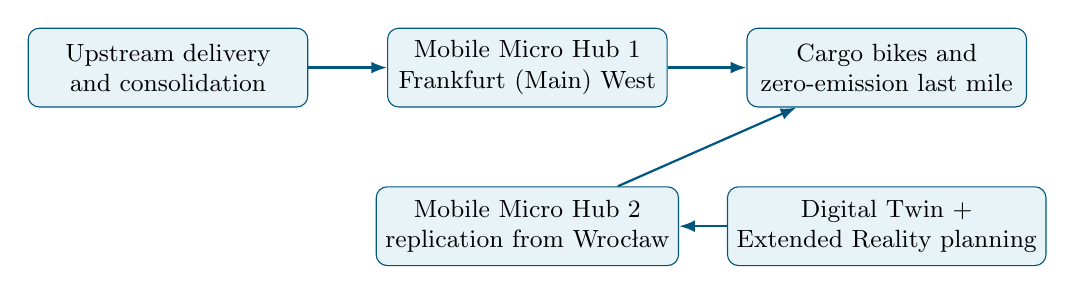
\begin{tikzpicture}[
  box/.style={rounded corners, draw=holmblue, fill=lightblue, align=center,
              minimum width=3.55cm, minimum height=1.0cm, font=\small},
  arr/.style={-{Latex[length=2mm]}, thick, draw=holmblue}
]
\node[box] (in) {Upstream delivery\\and consolidation};
\node[box, right=of in] (h1) {Mobile Micro Hub 1\\Frankfurt (Main) West};
\node[box, right=of h1] (last) {Cargo bikes and\\zero-emission last mile};
\node[box, below=of h1] (h2) {Mobile Micro Hub 2\\replication from Wrocław};
\node[box, below=of last] (digital) {Digital Twin +\\Extended Reality planning};
\draw[arr] (in) -- (h1);
\draw[arr] (h1) -- (last);
\draw[arr] (h2) -- (last);
\draw[arr] (digital) -- (h2);
\end{tikzpicture}
\vspace{3mm}
\begin{itemize}
  \item The first hub is implemented by DB InfraGO at Frankfurt (Main) West and builds on MOVE21 experience.
  \item The second hub transfers a solution from the leading city Wrocław and is planned with digital tools.
  \item Workshops, surveys, data-based site and concept development, and performance indicators connect demonstration with evaluation.
\end{itemize}
\source{HOLM, “HORIZON-Projekt NEXTLOGIC in Frankfurt am Main”.}
\end{frame}

\begin{frame}{HOLM's role within NEXTLOGIC}
\begin{columns}[T]
\column{0.49\textwidth}
\begin{block}{Institutional role}
\begin{itemize}
  \item HOLM leads the Frankfurt subproject.
  \item It coordinates DB InfraGO and the City of Frankfurt as associated partner.
  \item Frankfurt participates as a follower city, enabling structured learning and replication.
\end{itemize}
\end{block}
\column{0.47\textwidth}
\begin{block}{Knowledge-broker role}
\begin{itemize}
  \item Connects public authorities, infrastructure operators, carriers, research and users.
  \item Organises stakeholder workshops and surveys.
  \item Translates evidence into indicators, recommendations and transfer pathways.
  \item Builds on HOLM's open innovation and network-management experience.
\end{itemize}
\end{block}
\end{columns}
\source{HOLM, “Vision \& Strategie”; HOLM, “HORIZON-Projekt NEXTLOGIC in Frankfurt am Main”; HOLM campaign documentation.}
\end{frame}

\begin{frame}{How NEXTLOGIC can advance the research frontier}
\begin{enumerate}
  \item \textbf{From isolated cases to comparable evidence:} define a common indicator set for costs, service, emissions, space, acceptance and resilience.
  \item \textbf{From static maps to operational validation:} test candidate locations with real access constraints, time windows, charging and staffing requirements.
  \item \textbf{From single-carrier pilots to governance:} evaluate shared-use and public--private arrangements explicitly.
  \item \textbf{From deployment to replication:} use the Wrocław transfer and Digital Twin/Extended Reality tools to document what is context-specific.
  \item \textbf{From model output to decisions:} combine optimisation with workshops, surveys and transparent trade-offs.
\end{enumerate}
\begin{alertblock}{Research contribution}
Frankfurt can function as a living laboratory linking location science, implementation practice and urban governance.
\end{alertblock}
\end{frame}

\begin{frame}{Open questions for the Frankfurt work package}
\begin{itemize}
  \item What demand data are available at sufficiently fine spatial and temporal resolution?
  \item How should emissions be compared when upstream detours, hub handling and cargo-bike operations are included?
  \item Which ownership and access model is viable for two mobile hubs over time?
  \item How do residents, retailers, carriers and drivers value public-space, service and safety trade-offs?
  \item How robust are results under seasonal demand, delivery peaks, weather and construction-related access changes?
  \item Which indicators make replication decisions transparent across cities?
\end{itemize}
\source{Synthesis of the provided literature, Frankfurt data overview and NEXTLOGIC project description.}
\end{frame}

\begin{frame}{Conclusions}
\footnotesize
\begin{block}{What is established}
Microdepots are a credible mechanism for urban freight consolidation and a mode shift toward low-emission last-mile delivery.
\end{block}
\begin{block}{What remains conditional}
Impacts depend on location, demand density, access, fleet, ownership, collaboration and the wider network; evidence is still heterogeneous.
\end{block}
\begin{block}{Why NEXTLOGIC matters}
The Frankfurt demonstrator combines two mobile hubs, digital planning, stakeholder participation and performance evaluation---precisely the ingredients needed to move from promising pilots to transferable evidence.
\end{block}
\begin{block}{HOLM's added value}
HOLM provides the coordination, network and innovation-management capacity that connects research, infrastructure, city policy and implementation.
\end{block}
\end{frame}

\begin{frame}[allowframebreaks]{Selected sources}
\footnotesize
\begin{thebibliography}{99}
\bibitem{Katsela2022}
Katsela, K., Kourounioti, I., Thoen, S., Winkenbach, M. \& de Koster, R. (2022).
\newblock Defining Urban Freight Microhubs: A Case Study Analysis.
\newblock \emph{Sustainability}, 14, 532. \url{https://doi.org/10.3390/su14010532}

\bibitem{Stokkink2025}
Stokkink, P. \& Geroliminis, N. (2025).
\newblock On the optimal micro-hub locations in a multi-modal last-mile delivery system.
\newblock Provided article, Elsevier, open access.

\bibitem{Mauch}
Mauch, M. et al. (2019).
\newblock \emph{logSPAZE: Micro-Hubs für die urbane Logistik}.
\newblock Fraunhofer / Landeshauptstadt Stuttgart, provided report.

\bibitem{HOLMCampaign}
HOLM \& Radlogistik Verband Deutschland (2021).
\newblock \emph{Deutschland sucht das Super-Mikrodepot}.
\newblock Ergebnispapier der digitalen Kampagne.

\bibitem{HOLMNextlogic}
House of Logistics and Mobility (HOLM) GmbH (2026).
\newblock \emph{HORIZON-Projekt NEXTLOGIC in Frankfurt am Main}.
\newblock Provided HTML article, \url{https://frankfurt-holm.de/unsere-leistungen/innovations-netzwerkmanagement/projekte/nextlogic/}

\bibitem{HOLMVision}
House of Logistics and Mobility (HOLM) GmbH (2026).
\newblock \emph{Vision \& Strategie}.
\newblock Provided HTML article.

\bibitem{EUObservatory}
European Commission, Urban Mobility Observatory (n.d.).
\newblock \emph{Microhubs as the future of last-mile logistics}.
\newblock Provided HTML article.

\bibitem{DataSources}
Provided project document (2026).
\newblock \emph{Data sources for the study area Frankfurt am Main}.
\end{thebibliography}
\end{frame}

\end{document}
